\newcommand{\embed}[1]{\mathcal{#1}}  %% may be worth moving to mcs.tex?

\hyperdef{planar}{graphs}{\chapter{Planar Graphs}\label{planar-graphs-chapter}}

\section{Drawing Graphs in the Plane}

Here are three dogs and three houses.

%\mfigure{!}{1.5in}{dog-houses}
\begin{center}
\setlength{\unitlength}{2000sp}%{3947sp}%
%
\begingroup\makeatletter\ifx\SetFigFont\undefined%
\gdef\SetFigFont#1#2#3#4#5{%
  \reset@font\fontsize{#1}{#2pt}%
  \fontfamily{#3}\fontseries{#4}\fontshape{#5}%
  \selectfont}%
\fi\endgroup%
\begin{picture}(5424,2793)(1039,-3742)
%\thinlines
{\color[rgb]{0,0,0}\put(1201,-1861){\framebox(450,450){}}
}%
{\color[rgb]{0,0,0}\put(1051,-1411){\line( 1, 0){750}}
\put(1801,-1411){\line(-2, 3){300}}
\put(1501,-961){\line(-1,-1){450}}
}%
{\color[rgb]{0,0,0}\put(3451,-1861){\framebox(450,450){}}
}%
{\color[rgb]{0,0,0}\put(3301,-1411){\line( 1, 0){750}}
\put(4051,-1411){\line(-2, 3){300}}
\put(3751,-961){\line(-1,-1){450}}
}%
{\color[rgb]{0,0,0}\put(5851,-1861){\framebox(450,450){}}
}%
{\color[rgb]{0,0,0}\put(5701,-1411){\line( 1, 0){750}}
\put(6451,-1411){\line(-2, 3){300}}
\put(6151,-961){\line(-1,-1){450}}
}%
\put(3451,-3661){\makebox(0,0)[lb]{\smash{{\SetFigFont{17}{20.4}{\rmdefault}{\bfdefault}{\updefault}{\color[rgb]{0,0,0}Dog}%
}}}}
\put(5851,-3661){\makebox(0,0)[lb]{\smash{{\SetFigFont{17}{20.4}{\rmdefault}{\bfdefault}{\updefault}{\color[rgb]{0,0,0}Dog}%
}}}}
\put(1201,-3661){\makebox(0,0)[lb]{\smash{{\SetFigFont{17}{20.4}{\rmdefault}{\bfdefault}{\updefault}{\color[rgb]{0,0,0}Dog}%
}}}}
\end{picture}%

\end{center}

Can you find a path from each dog to each house such that no
two paths intersect?

A \emph{quadapus} is a little-known animal similar to an octopus,
but with four arms.  Here are five quadapi resting on the seafloor:

%%%%%%%%%%%%.fig

%\mfigure{!}{2in}{figures/quadapi.pdf}
\begin{center}
\setlength{\unitlength}{2000sp}%{3947sp}%
%
\begingroup\makeatletter\ifx\SetFigFont\undefined%
\gdef\SetFigFont#1#2#3#4#5{%
  \reset@font\fontsize{#1}{#2pt}%
  \fontfamily{#3}\fontseries{#4}\fontshape{#5}%
  \selectfont}%
\fi\endgroup%
\begin{picture}(11049,5049)(589,-5248)
{\color[rgb]{0,0,0}%\thinlines
\put(4688,-1673){\oval(524,524)}
}%
{\color[rgb]{0,0,0}\put(1913,-2948){\oval(524,524)}
}%
{\color[rgb]{0,0,0}\put(4538,-3923){\oval(524,524)}
}%
{\color[rgb]{0,0,0}\put(7838,-3098){\oval(524,524)}
}%
{\color[rgb]{0,0,0}\put(9713,-1748){\oval(524,524)}
}%
{\color[rgb]{0,0,0}\put(4426,-1636){\line(-1, 0){900}}
\multiput(3526,-1636)(-2.67857,-8.03571){57}{\makebox(1.6667,11.6667){\SetFigFont{5}{6}{\rmdefault}{\mddefault}{\updefault}.}}
\put(3376,-2086){\line(-1, 0){750}}
}%
{\color[rgb]{0,0,0}\put(4951,-1711){\line( 5,-3){893.382}}
\put(5851,-2236){\line( 5, 6){442.623}}
\put(6301,-1711){\line( 2,-3){300}}
}%
{\color[rgb]{0,0,0}\multiput(1876,-2686)(1.37838,8.27027){101}{\makebox(1.6667,11.6667){\SetFigFont{5}{6}{\rmdefault}{\mddefault}{\updefault}.}}
\put(2026,-1861){\line( 5, 2){685.345}}
\put(2701,-1561){\line( 0, 1){375}}
}%
{\color[rgb]{0,0,0}\put(2176,-2986){\line( 5, 2){750}}
\put(2926,-2686){\line( 5,-6){510.246}}
\put(3451,-3286){\line( 6, 1){450}}
}%
{\color[rgb]{0,0,0}\put(1951,-3211){\line(-1,-2){300}}
\put(1651,-3811){\line( 5,-6){375}}
\put(2026,-4261){\line( 3, 2){450}}
}%
{\color[rgb]{0,0,0}\put(1651,-2986){\line(-6, 5){612.295}}
\put(1051,-2461){\line(-5,-6){442.623}}
\multiput(601,-2986)(2.02703,-8.10811){75}{\makebox(1.6667,11.6667){\SetFigFont{5}{6}{\rmdefault}{\mddefault}{\updefault}.}}
}%
{\color[rgb]{0,0,0}\multiput(4501,-3661)(1.37838,8.27027){101}{\makebox(1.6667,11.6667){\SetFigFont{5}{6}{\rmdefault}{\mddefault}{\updefault}.}}
\put(4651,-2836){\line( 5, 2){685.345}}
\put(5326,-2536){\line( 0, 1){375}}
}%
{\color[rgb]{0,0,0}\put(4801,-3961){\line( 5, 2){750}}
\put(5551,-3661){\line( 5,-6){510.246}}
\put(6076,-4261){\line( 6, 1){450}}
}%
{\color[rgb]{0,0,0}\put(4576,-4186){\line(-1,-2){300}}
\put(4276,-4786){\line( 5,-6){375}}
\put(4651,-5236){\line( 3, 2){450}}
}%
{\color[rgb]{0,0,0}\put(7576,-3061){\line(-1, 0){900}}
\multiput(6676,-3061)(-2.67857,-8.03571){57}{\makebox(1.6667,11.6667){\SetFigFont{5}{6}{\rmdefault}{\mddefault}{\updefault}.}}
\put(6526,-3511){\line(-1, 0){750}}
}%
{\color[rgb]{0,0,0}\put(7876,-2836){\line(-1, 1){375}}
\put(7501,-2461){\line( 4, 3){600}}
\put(8101,-2011){\line( 0, 1){450}}
}%
{\color[rgb]{0,0,0}\put(8101,-3136){\line( 5,-3){893.382}}
\put(9001,-3661){\line( 5, 6){442.623}}
\put(9451,-3136){\line( 2,-3){300}}
}%
{\color[rgb]{0,0,0}\put(7876,-3361){\line(-2,-5){237.931}}
\put(7651,-3961){\line( 1,-1){600}}
}%
{\color[rgb]{0,0,0}\put(9751,-1486){\line(-1, 1){375}}
\put(9376,-1111){\line( 4, 3){600}}
\put(9976,-661){\line( 0, 1){450}}
}%
{\color[rgb]{0,0,0}\put(9976,-1786){\line( 5,-3){893.382}}
\put(10876,-2311){\line( 5, 6){442.623}}
\put(11326,-1786){\line( 2,-3){300}}
}%
{\color[rgb]{0,0,0}\put(9751,-2011){\line(-2,-5){237.931}}
\put(9526,-2611){\line( 1,-1){600}}
}%
{\color[rgb]{0,0,0}\put(9451,-1711){\line(-5,-1){677.885}}
\put(8776,-1861){\line(-2, 3){692.308}}
\put(8101,-811){\line(-5,-1){1572.115}}
}%
{\color[rgb]{0,0,0}\put(4651,-1936){\line(-1,-4){339.706}}
\put(4276,-3286){\line(-4,-1){1358.823}}
\multiput(2926,-3661)(-1.37838,-8.27027){101}{\makebox(1.6667,11.6667){\SetFigFont{5}{6}{\rmdefault}{\mddefault}{\updefault}.}}
}%
{\color[rgb]{0,0,0}\put(4276,-3886){\line(-3,-2){761.538}}
\multiput(3526,-4411)(2.03287,-8.13149){103}{\makebox(1.6667,11.6667){\SetFigFont{5}{6}{\rmdefault}{\mddefault}{\updefault}.}}
}%
{\color[rgb]{0,0,0}\multiput(4726,-1411)(-1.37387,8.24324){91}{\makebox(1.6667,11.6667){\SetFigFont{5}{6}{\rmdefault}{\mddefault}{\updefault}.}}
\put(4651,-661){\line( 2,-1){1290}}
\put(5926,-1336){\line( 6,-1){1277.027}}
}%
\end{picture}%

\end{center}

Can each quadapus simultaneously shake hands with every other in such a
way that no arms cross?

Informally, a \term{planar graph} is a graph that can be drawn in the
plane so that no edges cross, as in a map of showing the borders of
countries or states.  Thus, these two puzzles are asking whether the
graphs below are planar; that is, whether they can be redrawn so that no
edges cross.  The first graph is called the \term{complete bipartite
  graph}, \idx{$K_{3,3}$}, and the second is \idx{$K_5$}.

%\mfigure{!}{1.5in}{figures/nonplanar.pdf}
\begin{center}
\setlength{\unitlength}{3000sp}%{3947sp}%
%
\begingroup\makeatletter\ifx\SetFigFont\undefined%
\gdef\SetFigFont#1#2#3#4#5{%
  \reset@font\fontsize{#1}{#2pt}%
  \fontfamily{#3}\fontseries{#4}\fontshape{#5}%
  \selectfont}%
\fi\endgroup%
\begin{picture}(7366,2266)(2318,-2244)
{\color[rgb]{0,0,0}%\thinlines
\put(2401,-661){\circle{150}}
}%
{\color[rgb]{0,0,0}\put(4726,-661){\circle{150}}
}%
{\color[rgb]{0,0,0}\put(3601,-661){\circle{150}}
}%
{\color[rgb]{0,0,0}\put(3601,-2161){\circle{150}}
}%
{\color[rgb]{0,0,0}\put(2401,-2161){\circle{150}}
}%
{\color[rgb]{0,0,0}\put(4801,-2161){\circle{150}}
}%
{\color[rgb]{0,0,0}\put(8401,-61){\circle{150}}
}%
{\color[rgb]{0,0,0}\put(7201,-961){\circle{150}}
}%
{\color[rgb]{0,0,0}\put(9601,-961){\circle{150}}
}%
{\color[rgb]{0,0,0}\put(7801,-2161){\circle{150}}
}%
{\color[rgb]{0,0,0}\put(9001,-2161){\circle{150}}
}%
{\color[rgb]{0,0,0}\put(2401,-661){\line( 0,-1){1500}}
\put(2401,-2161){\line( 4, 5){1200}}
\put(3601,-661){\line( 4,-5){1200}}
\put(4801,-2161){\line( 0, 1){1500}}
\put(4726,-661){\line(-3,-4){1125}}
\put(3601,-2161){\line(-4, 5){1200}}
}%
{\color[rgb]{0,0,0}\put(3601,-661){\line( 0,-1){1500}}
}%
{\color[rgb]{0,0,0}\put(2401,-661){\line( 5,-3){2426.471}}
}%
{\color[rgb]{0,0,0}\put(4726,-661){\line(-3,-2){2301.923}}
}%
{\color[rgb]{0,0,0}\put(7201,-961){\line( 1,-2){600}}
\put(7801,-2161){\line( 1, 0){1200}}
\put(9001,-2161){\line( 1, 2){600}}
\put(9601,-961){\line(-4, 3){1200}}
\put(8401,-61){\line(-4,-3){1200}}
\put(7201,-961){\line( 1, 0){2400}}
\put(9601,-961){\line(-3,-2){1800}}
\put(7801,-2161){\line( 1, 4){529.412}}
\put(8401,-61){\line( 1,-4){529.412}}
}%
{\color[rgb]{0,0,0}\put(9001,-2161){\line(-3, 2){1800}}
}%
\end{picture}%

\end{center}

In each case, the answer is, ``No--- but almost!''  In fact, each drawing
\emph{would} be possible if any single edge were removed.

Planar graphs have applications in circuit layout and are helpful in
displaying graphical data, for example, program flow charts, organizational
charts, and scheduling conflicts.  We will treat them as a recursive data
type and use structural induction to establish their basic properties.
Then we'll be able to describe a simple recursive procedure to color any
planar graph with \emph{five} colors, and also prove that there is no
uniform way to place $n$ satellites around the globe unless $n = 4,6,8,12$,
or $20$.

\iffalse
We will use them to
prove a wonderful mathematical fact that was first proved by the ancient
Greeks.
\fi

\iffalse
One is rooted in human pyschology: many kinds of information can
be presented as a graph (family relations, chemical structures, computer
data structures, contact data for study of disease spread, flow of cash in
money laundering trials, etc.).  Big graphs are typically incomprehensible
messes, but planar graphs are relatively easy for humans to grasp since
there are no crisscrossing edges.  \fi

\textbox{\noindent 
When wires are arranged on a surface, like a circuit board or microchip,
crossings require troublesome three-dimensional structures.  When Steve
Wozniak designed the disk drive for the early Apple II computer, he
struggled mightly to achieve a nearly planar design:
%
\begin{quotation}
\noindent For two weeks, he worked late each night to make a satisfactory
design.  When he was finished, he found that if he moved a connector he
could cut down on feedthroughs, making the board more reliable.  To make
that move, however, he had to start over in his design.  This time it only
took twenty hours. He then saw another feedthrough that could be
eliminated, and again started over on his design.  "The final design was
generally recognized by computer engineers as brilliant and was by
engineering aesthetics beautiful.  Woz later said, 'It's something you can
only do if you're the engineer and the PC board layout person yourself.
That was an artistic layout.  The board has virtually no
feedthroughs.'"\footnote{From apple2history.org which in turn quotes
\textit{Fire in the Valley} by Freiberger and Swaine.}
\end{quotation}
}

\iffalse
Finally, as we'll see shortly, planar graphs reveal a fundamental
truth about the structure of our three-dimensional world.
\fi

\section{Continuous \& Discrete Faces}

Planar graphs are graphs that can be drawn in the plane ---like familiar
maps of countries or states.  ``Drawing'' the graph means that each vertex
of the graph corresponds to a distinct point in the plane, and if two
vertices are adjacent, their vertices are connected by a smooth,
non-self-intersecting curve.  None of the curves may ``cross'' ---the only
points that may appear on more than one curve are the vertex points.
These curves are the boundaries of connected regions of the plane called
the \emph{continuous faces} of the drawing.

For example, the drawing in Figure~\ref{fig:continuous-faces} has four
continuous faces.
\begin{figure}[h]
\centering 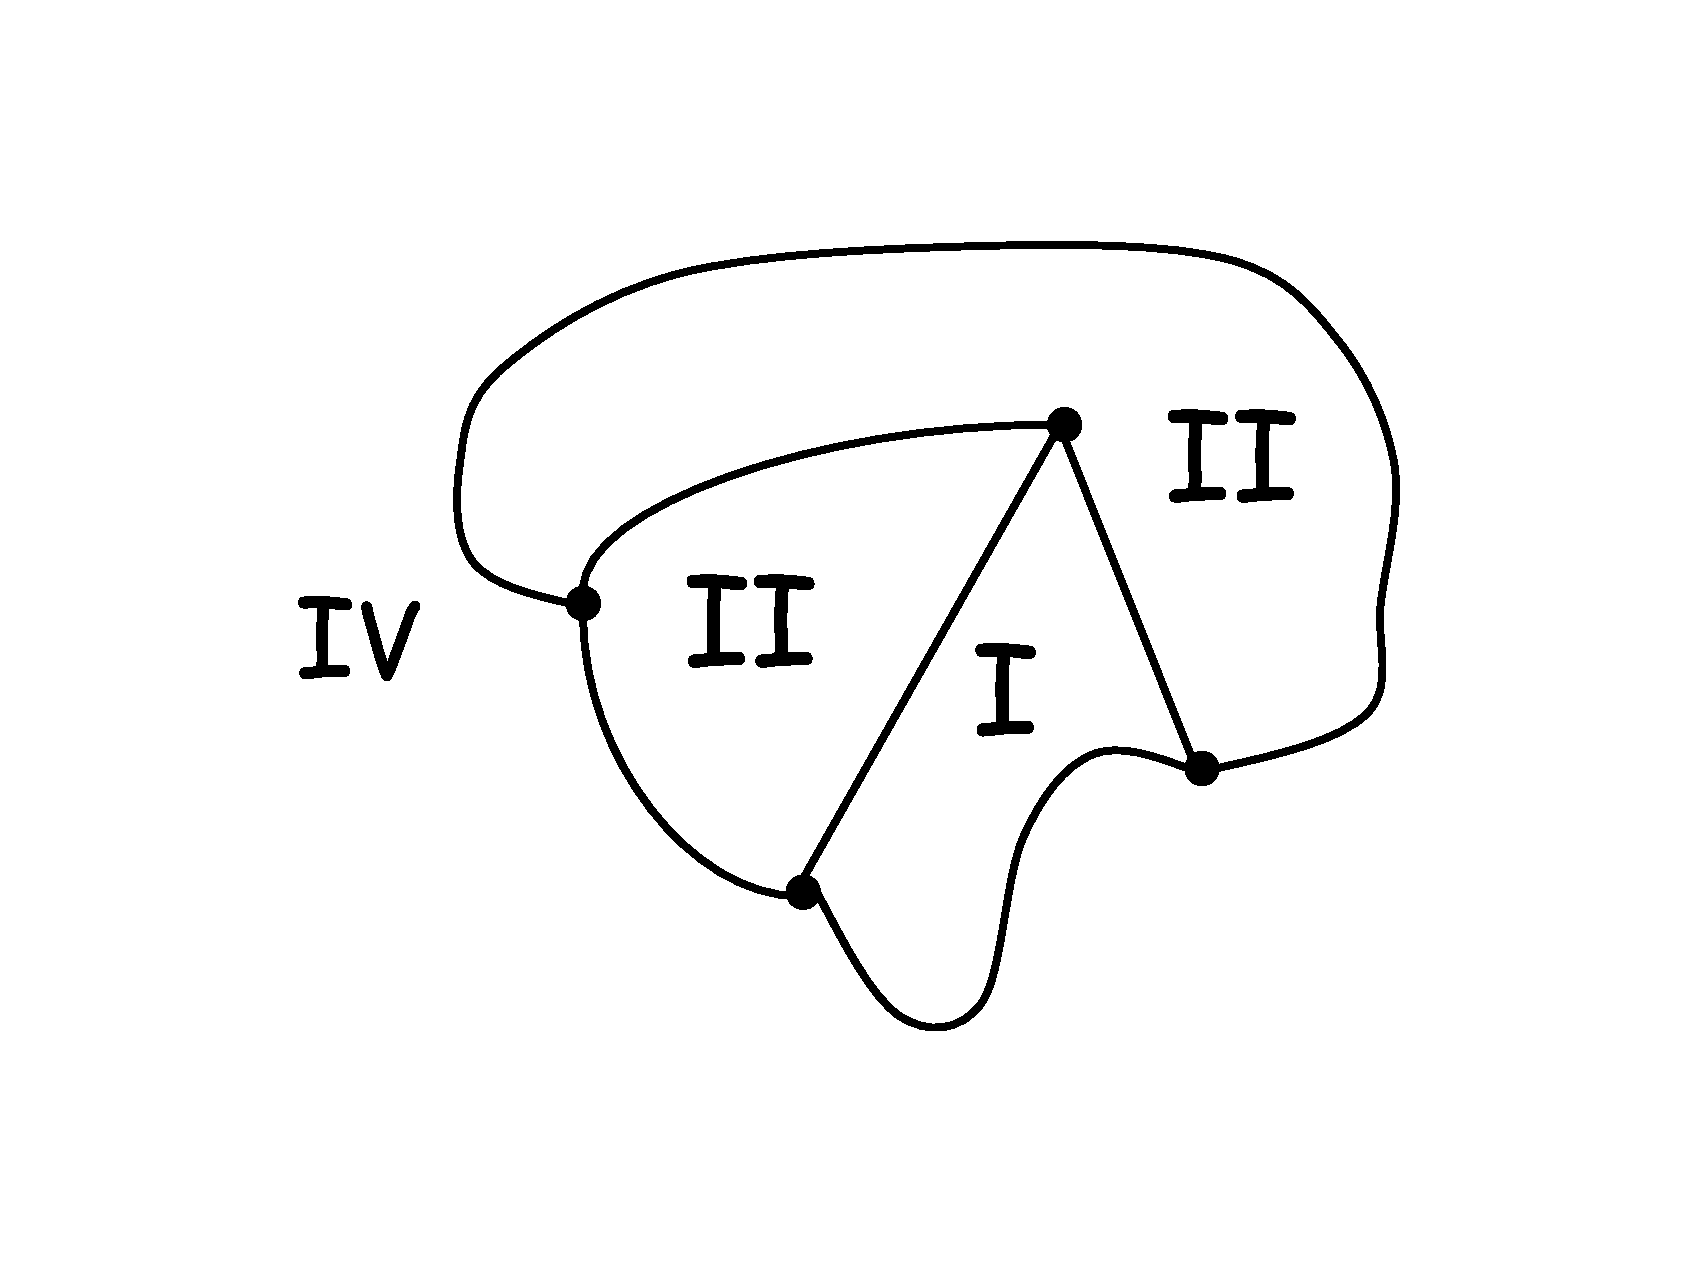
\includegraphics[height=2in]{figures/continuous-faces}
\caption{A Planar Drawing with Four Faces.}
\label{fig:continuous-faces}
\end{figure}
Face IV, which extends off to infinity in all directions, is called the
\term{outside face}.

This definition of planar graphs is perfectly precise, but completely
unsatisfying: it invokes smooth curves and continuous regions of the plane
to define a property of a discrete data type.  So the first thing we'd
like to find is a discrete data type that represents planar drawings.

The clue to how to do this is to notice that the vertices along the
boundary of each of the faces in Figure~\ref{fig:continuous-faces} form a
simple cycle.  For example, labeling the vertices as in
Figure~\ref{fig:continuous-cycles}, the simple cycles for the face
boundaries are
\[
\mathtt{abca}\qquad \mathtt{abda}\qquad \mathtt{bcdb}\qquad \mathtt{acda}.
\]
Since every edge in the drawing appears on the boundaries of exactly two
continuous faces, every edge of the simple graph appears on exactly two of
the simple cycles.

\begin{figure}
\centering 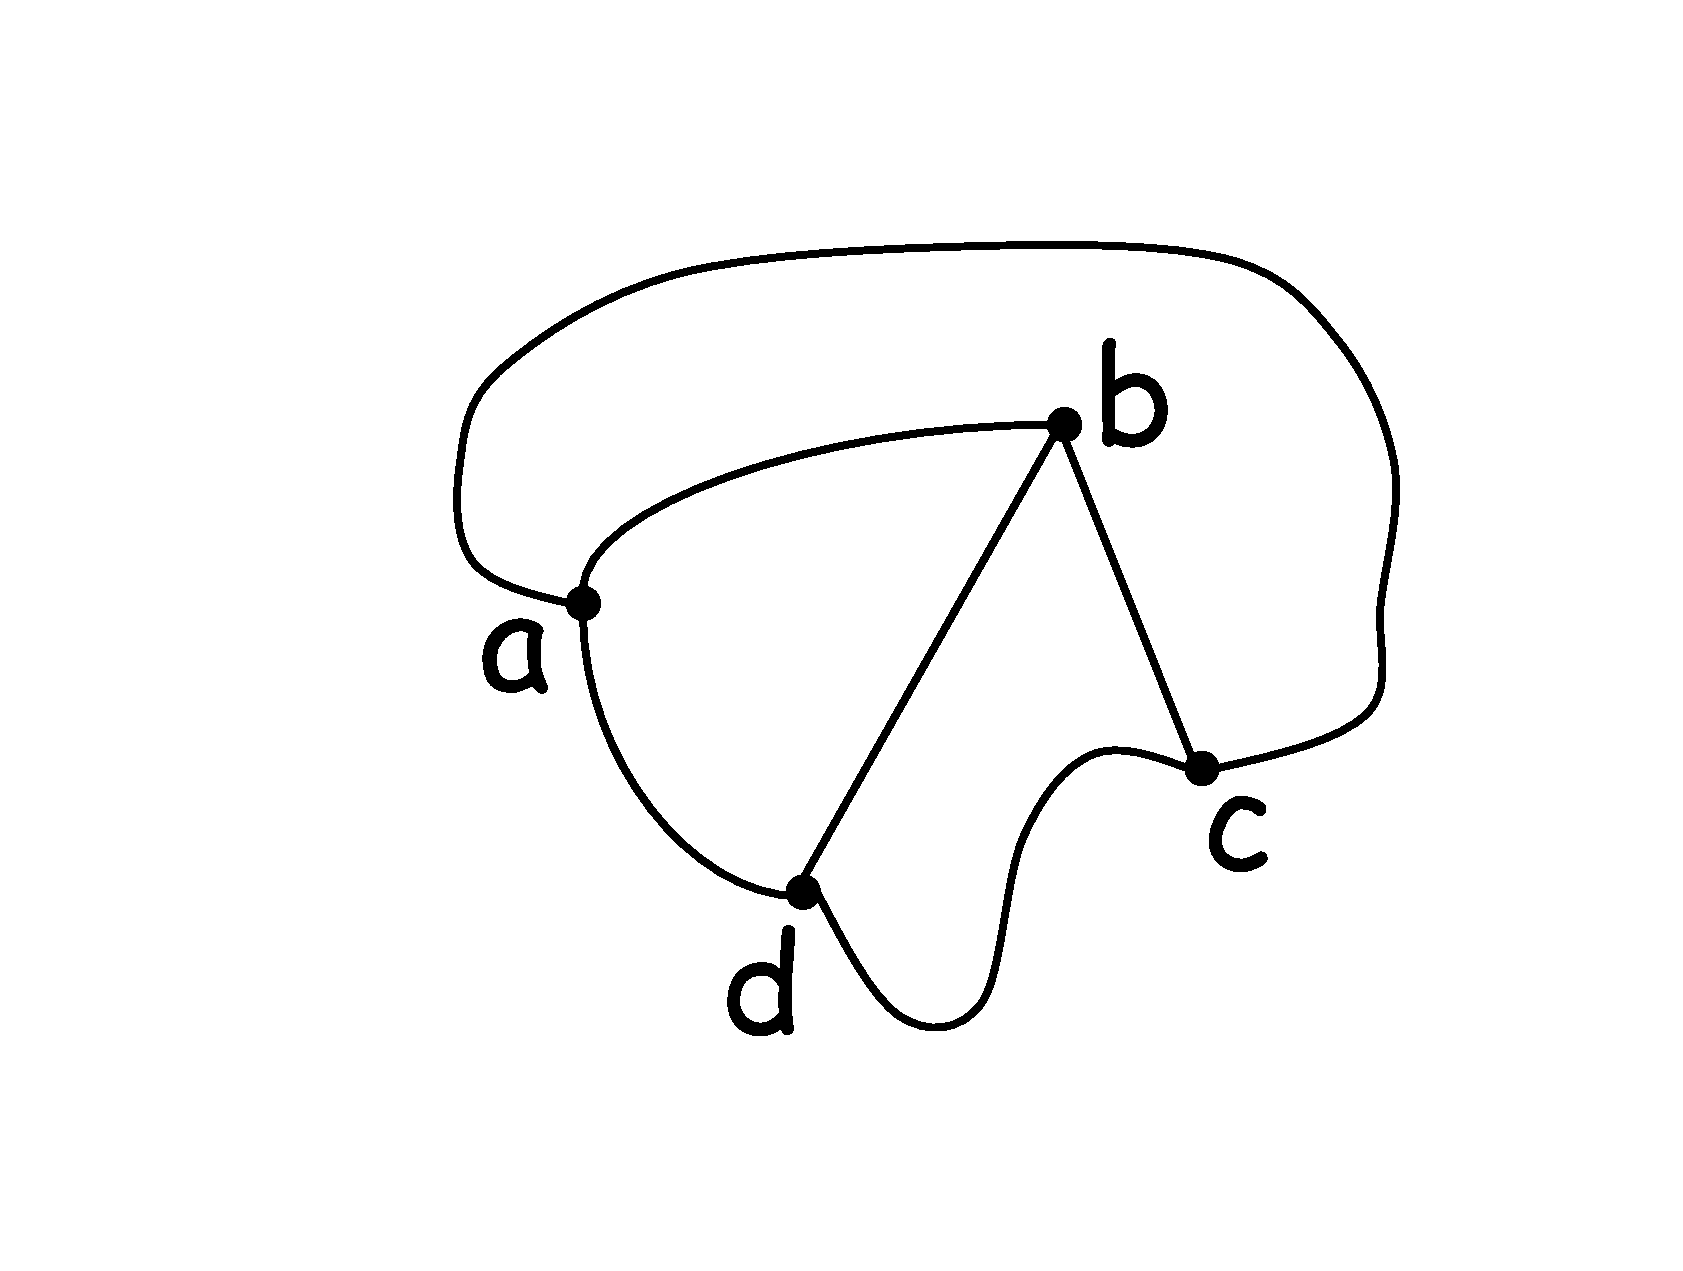
\includegraphics[height=2in]{figures/continuous-cycles}
\caption{The Drawing with Labelled Vertices.}
\label{fig:continuous-cycles}
\end{figure}

Vertices around the boundaries of states and countries in an ordinary map
are always simple cycles, but oceans are slightly messier.  The ocean
boundary is the set of all boundaries of islands and continents in the
ocean; it is a \emph{set} of simple cycles (this can happen for countries
too ---like Bangladesh).  But this happens because islands (and the two
parts of Bangladesh) are not connected to each other.  So we can dispose
of this complication by treating each connected component separately.

But general planar graphs, even when they are connected, may be a bit more
complicated than maps.  For example a planar graph may have a
``\idx{bridge},'' as in Figure~\ref{fig:bridge}.
\begin{figure}[h]
\centering 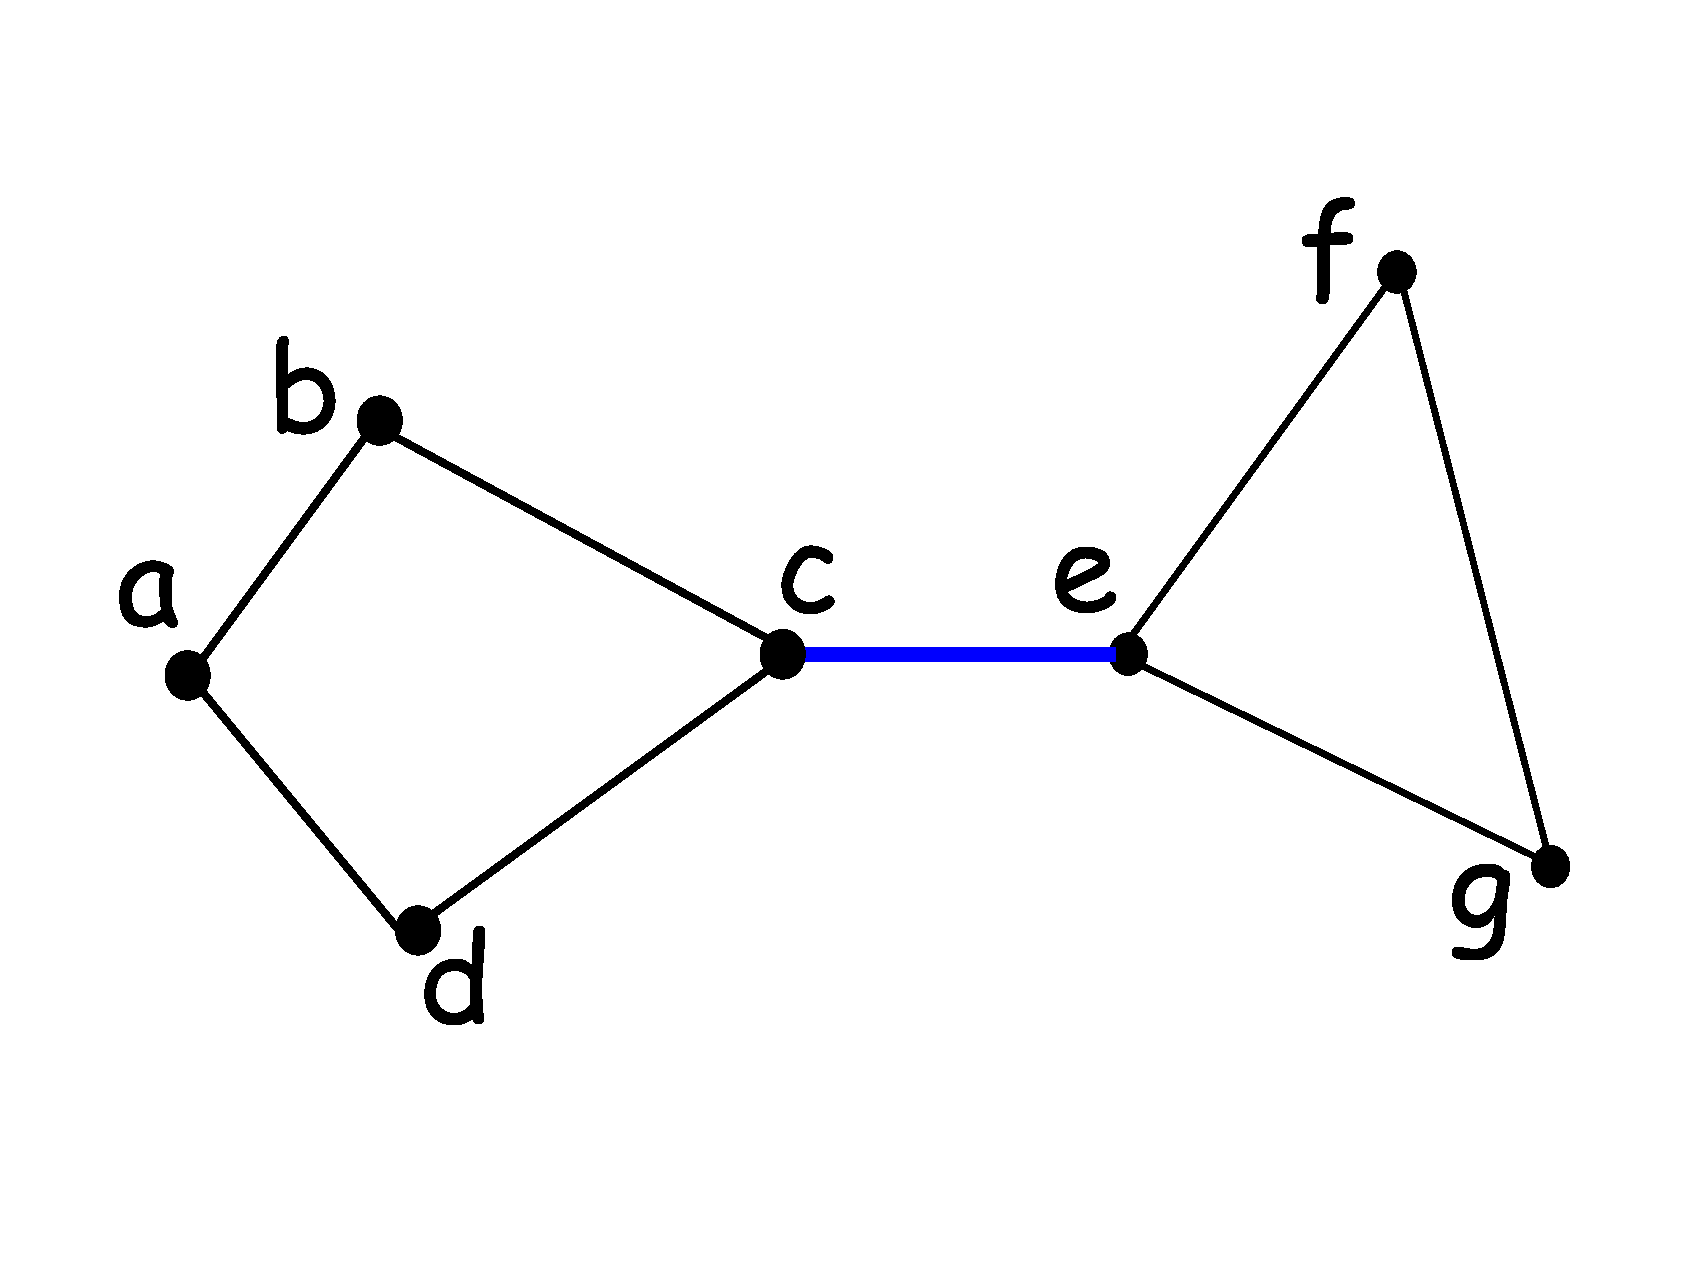
\includegraphics[height=2in]{figures/edge-twice-same-face}
\caption{A Planar Drawing with a \emph{Bridge}.}
\label{fig:bridge}
\end{figure}
Now the cycle around the outer face is
\[
\mathtt{abcefgecda}.
\]
This is not a simple cycle, since it has to traverse the bridge
$\edge{c}{e}$ twice.

Planar graphs may also have ``\idx{dongles},'' as in
Figure~\ref{fig:dongle}.
\begin{figure}[h]
\centering 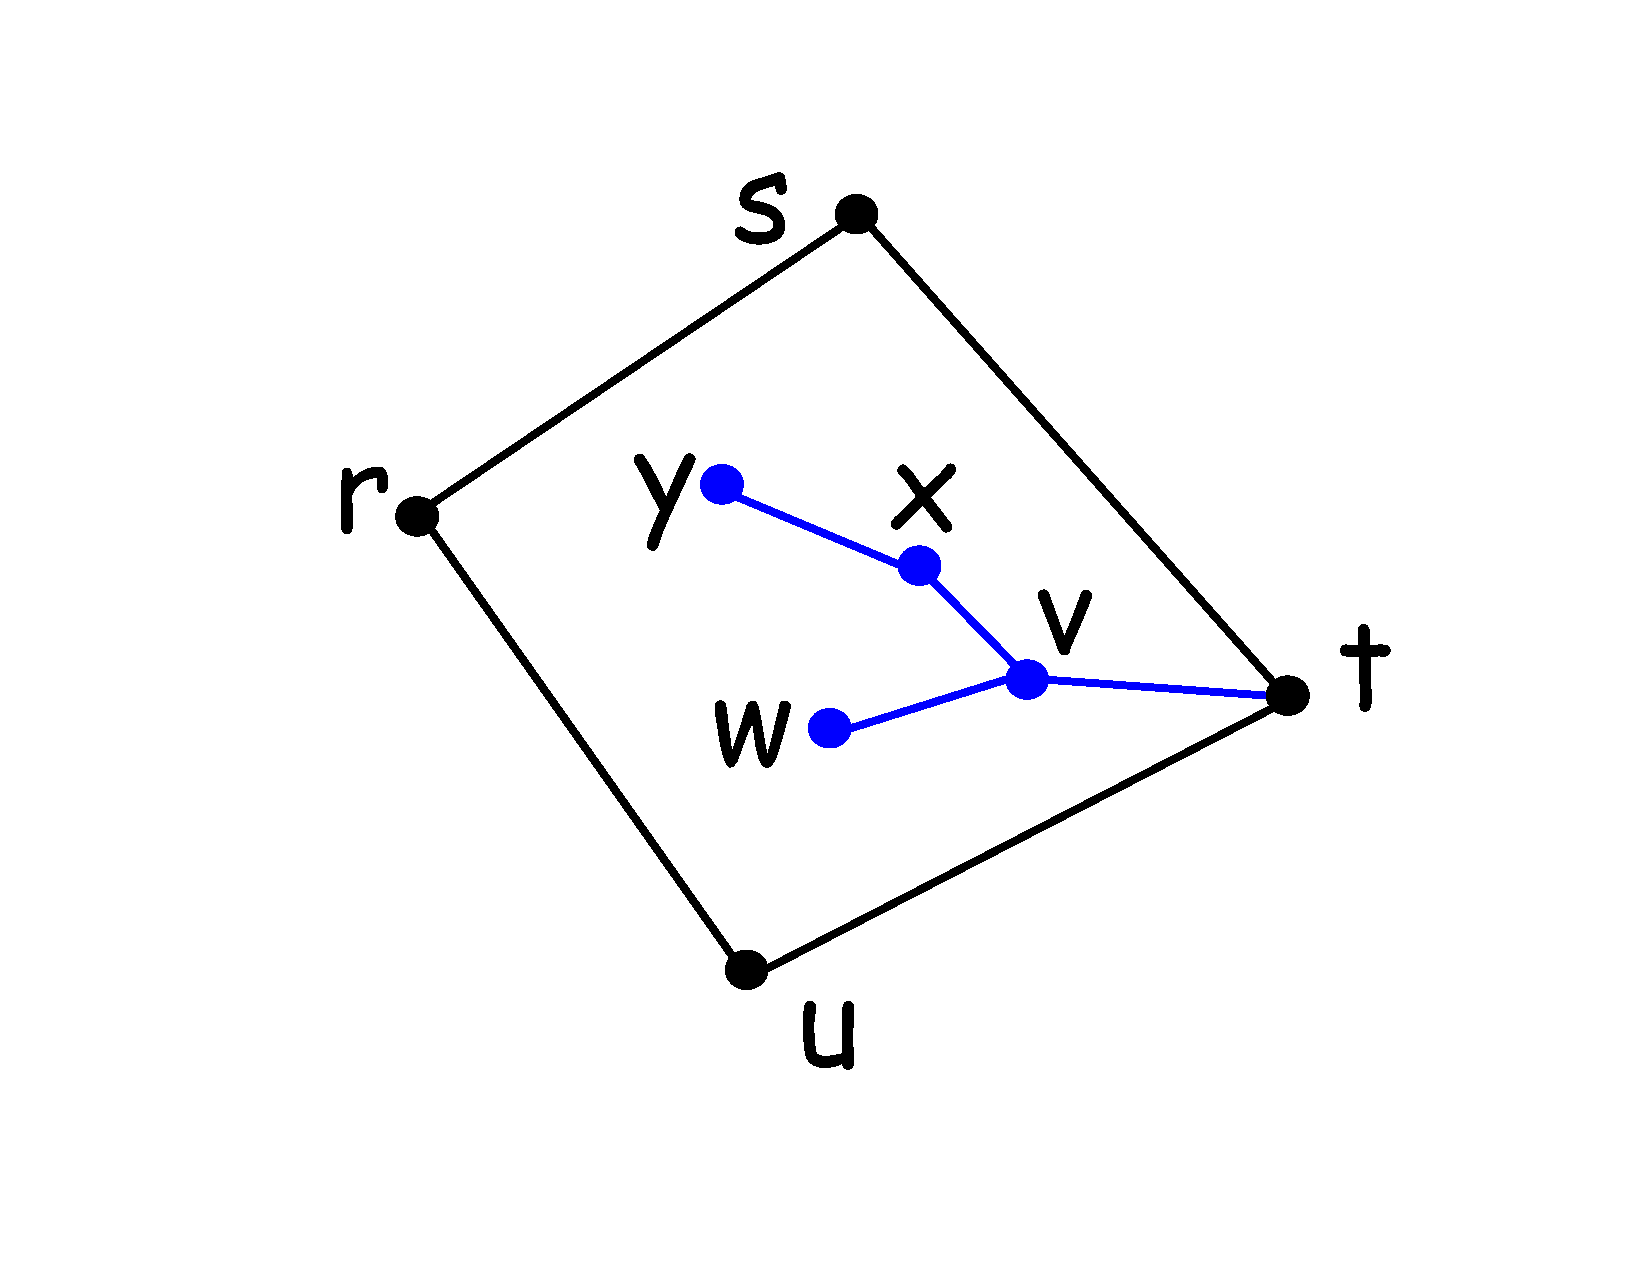
\includegraphics[height=2in]{figures/dongle-face}
\caption{A Planar Drawing with a \emph{Dongle}.}
\label{fig:dongle}
\end{figure}
Now the cycle around the inner face is
\[
\mathtt{rstvxyxvwvtur},
\]
because it has to traverse \emph{every} edge of the dongle twice ---once
``coming'' and once ``going.''

But bridges and dongles are really the only complications, which leads
us to the discrete data type of \term{planar embeddings} that we can use
in place of continuous planar drawings.  Namely, we'll define a planar
embedding recursively to be the set of boundary-tracing cycles we could
get drawing one edge after another.

\iffalse  FAILED ATTEMPT TO AVOID RECURSIVE DEF
One property of the set of boundary-tracing cycles is that every
edge is traversed a total of two times by cycles in the set.  This is
almost enough to pin down exactly when a set of cycles are the
boundary-tracing cycles of a planar drawing, but not quite.  To illustrate
the remaining technicality, look at Figure~\ref{fig:bridge} showing a
bridge.  This graph has three faces described by the boundary-tracing
cycles
\[
\mathtt{abcefgecda} \text{ (the outer face)} \qquad \mathtt{abcda}\qquad
\mathtt{efge}.
\]
But we might also split up the cycle for the outer boundary into two
cycles, giving the set of four cycles,
\[
\mathtt{abcecda}\qquad \mathtt{efge} \qquad \mathtt{abcda}\qquad
\mathtt{efge}
\]
We don't want to allow this kind of splitting up of genuine
boundary-tracing cycles, but the four cycles above do have the property
that every edge is still traversed exactly twice.  What's wrong with the
split cycles is that they backtrack on themselves when they don't have to
---backtracks should only occur when there's nowhere else to go.  More
precisely:
\begin{definition}
A cycle in a graph has a \emph{backtrack} at vertex $v$ iff it contains a
subsequence $w,v,w$ for some vertex, $w$.  A backtrack at $v$ is
\emph{necessary} iff $v$ has degree 1.
\end{definition}
Now we're finally ready to define planar embeddings.

Let $G$ be a connected graph.  A \emph{planar embedding} of $G$ is a
set\footnote{\label{C} There is one exception to this definition.  If $G$
is isomorphic to the simple cycle, $C_n$, then a planar drawing of $G$ has
an inner and an outer face with the \emph{same} simple cycle as the
boundary of both faces.  So we need to use two ``copies'' of this simple
cycle as the set of boundary cycles for this graph.  But since this is the
only situation in which two faces have the same boundary cycle, this
exception is better explained in a footnote than mentioned explicitly in
the definition.} of cycles called \emph{boundary cycles}, such that
every edge of $G$ is traversed either
\begin{itemize}
\item by exactly two boundary cycles that are simple cycles, or

\item twice by a single boundary cycle that only backtracks when
necessary.
\end{itemize}


we can eliminate having to reason about continuous faces by jumping
directly to what matters about a continuous face, namely, the sequence of
vertices on its boundary curves.  This sequence is an undirected cycle in
the graph.  We'll call such an undirected cycle a \emph{discrete face},
and refer to a graph along with its discrete faces as a \emph{planar
embedding} of the graph.

The simplest kind of discrete face comes from the boundary of a country in
a map drawing ---this would just be a simple cycle.  Also, since each edge
appears on a boundary between two countries, it is traversed a total of
two times by the set of discrete faces.

But maps of countries are only a special case of planar graph.  For
example, a tree can always be drawn in the plane.  Such a tree drawing
``divides'' the plane into just \emph{one} region whose ``boundary'' is
the points and curves in the drawing, and the cycle of successive vertices
around this boundary backtracks on itself at every leaf.  But still, every
edge in the tree is traversed exactly twice (coming and going) by the
boundary of the tree.  So a planar graph will always have a set of
discrete faces such that each edge of the graph is traversed a total of
two times by these faces.

It turns out, conversely, that if a graph has a set of discrete faces that
traverse each edge a total of two times, the graph is in fact planar.  The
idea behind this claim is to consider how the successive discrete faces
could be drawn in the plane one at a time, with each new face having all
its edges on the boundary of one of the regions created so far (and in the
right order) so it can be added without the need to cross another face.

\textbf{MORE NEEDED HERE.}

But the only way to really prove this requires working with continuous
faces and continuously connected planar regions, which we don't want to
get into.  So we'll just accept the following definition:

\begin{definition}
A \emph{planar embedding} of a graph, $G$, is a set of cycles of $G$ such
that every edge is traversed a total of two times by these cycles.  Each
cycle is called a \emph{face} of the embedding.  A graph is \emph{planar}
iff it has a planar embedding.
\end{definition}
\fi

\section{Planar Embeddings}

By thinking of the process of drawing a planar graph edge by edge, we can
give a useful recursive definition of planar embeddings.

\begin{definition}\label{embeddingdef}
A \term{planar embedding} of a \emph{connected} graph consists of a
nonempty set of cycles of the graph called the \term{discrete faces} of
the embedding.  Planar embeddings are defined recursively as follows:

\begin{itemize}

\item \textbf{Base case:} If $G$ is a graph consisting of a single vertex,
$v$, then a planar embedding of $G$ has one discrete face, namely the
length zero cycle, $v$.

\item \textbf{Constructor Case:} (split a face) Suppose $G$ is a
connected graph with a planar embedding, and suppose $a$ and $b$ are
distinct, nonadjacent vertices of $G$ that appear on some discrete face,
$\gamma$, of the planar embedding.  That is, $\gamma$ is a cycle of the form
\[
a \dots b \cdots a.
\]
Then the graph obtained by adding the edge $\edge{a}{b}$ to the edges of
$G$ has a planar embedding with the same discrete faces as $G$, except
that face $\gamma$ is replaced by the two discrete
faces\footnote{\label{C} There is one exception to this rule.  If $G$ is a
line graph beginning with $a$ and ending with $b$, then the cycles into
which $\gamma$ splits are actually the same.  That's because adding edge
$\edge{a}{b}$ creates a simple cycle graph, $C_n$, that divides the plane
into an ``inner'' and an ``outer'' region with the same border.  In order
to maintain the correspondence between continuous faces and discrete
faces, we have to allow two ``copies'' of this same cycle to count as
discrete faces.  But since this is the only situation in which two faces
are actually the same cycle, this exception is better explained in a
footnote than mentioned explicitly in the definition.}
\[
a\dots ba\quad \text{ and } \quad ab\cdots a, 
\]
as illustrated in Figure~\ref{fig:face-splitting}.

\begin{figure}[h]
\centering 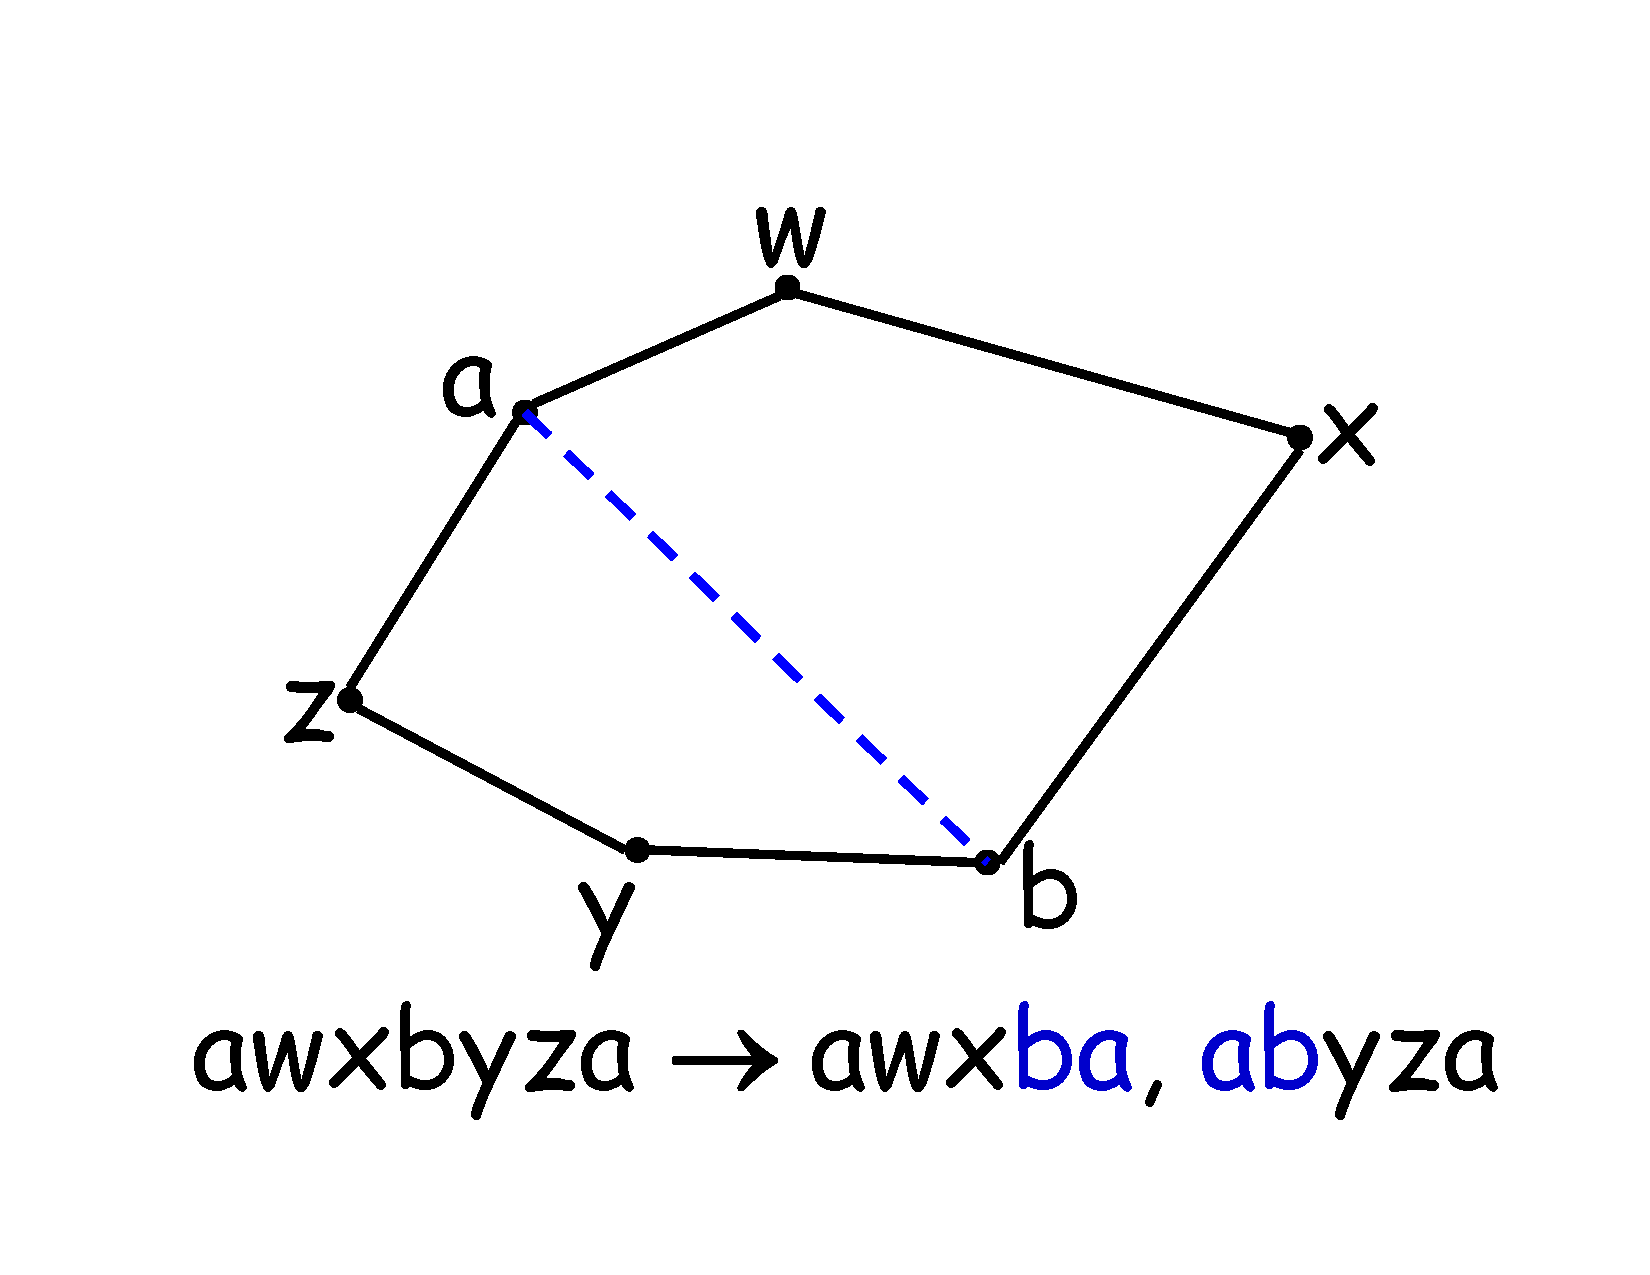
\includegraphics[height=2.5in]{figures/split-a-face}
\caption{The Split a Face Case.}
\label{fig:face-splitting}
\end{figure}

\item \textbf{Constructor Case:} (add a bridge) Suppose $G$ and $H$ are
connected graphs with planar embeddings and disjoint sets of vertices.
Let $a$ be a vertex on a discrete face, $\gamma$, in the embedding of
$G$.  That is, $\gamma$ is of the form
\[
a\dots a.
\]
Similarly, let $b$ be a vertex on a discrete face, $\delta$, in the
embedding of $H$, so $\delta$ is of the form
\[
b\cdots b.
\]
Then the graph obtained by connecting $G$ and $H$ with a new edge,
$\edge{a}{b}$, has a planar embedding whose discrete faces are the union of
the discrete faces of $G$ and $H$, except that faces $\gamma$ and $\delta$
are replaced by one new face
\[
a\dots ab\cdots ba.
\]
This is illustrated in Figure~\ref{fig:add-bridge}, where the faces of
$G$ and $H$ are:
\[
G: \set{\texttt{axyza},\ \texttt{axya},\ \texttt{ayza}}
    \qquad H: \set{\texttt{btuvwb},\ \texttt{btvwb},\ \texttt{tuvt}},
\]
and after adding the bridge $\edge{\texttt{a}}{\texttt{b}}$, there is a
single connected graph with faces
\[
\set{\texttt{axyz{\color{blue}ab}tuvw{\color{blue}ba}},\ 
         \texttt{axya},\ \texttt{ayza},\ \texttt{btvwb},\ \texttt{tuvt}}.
\]
\begin{figure}[h]
\centering 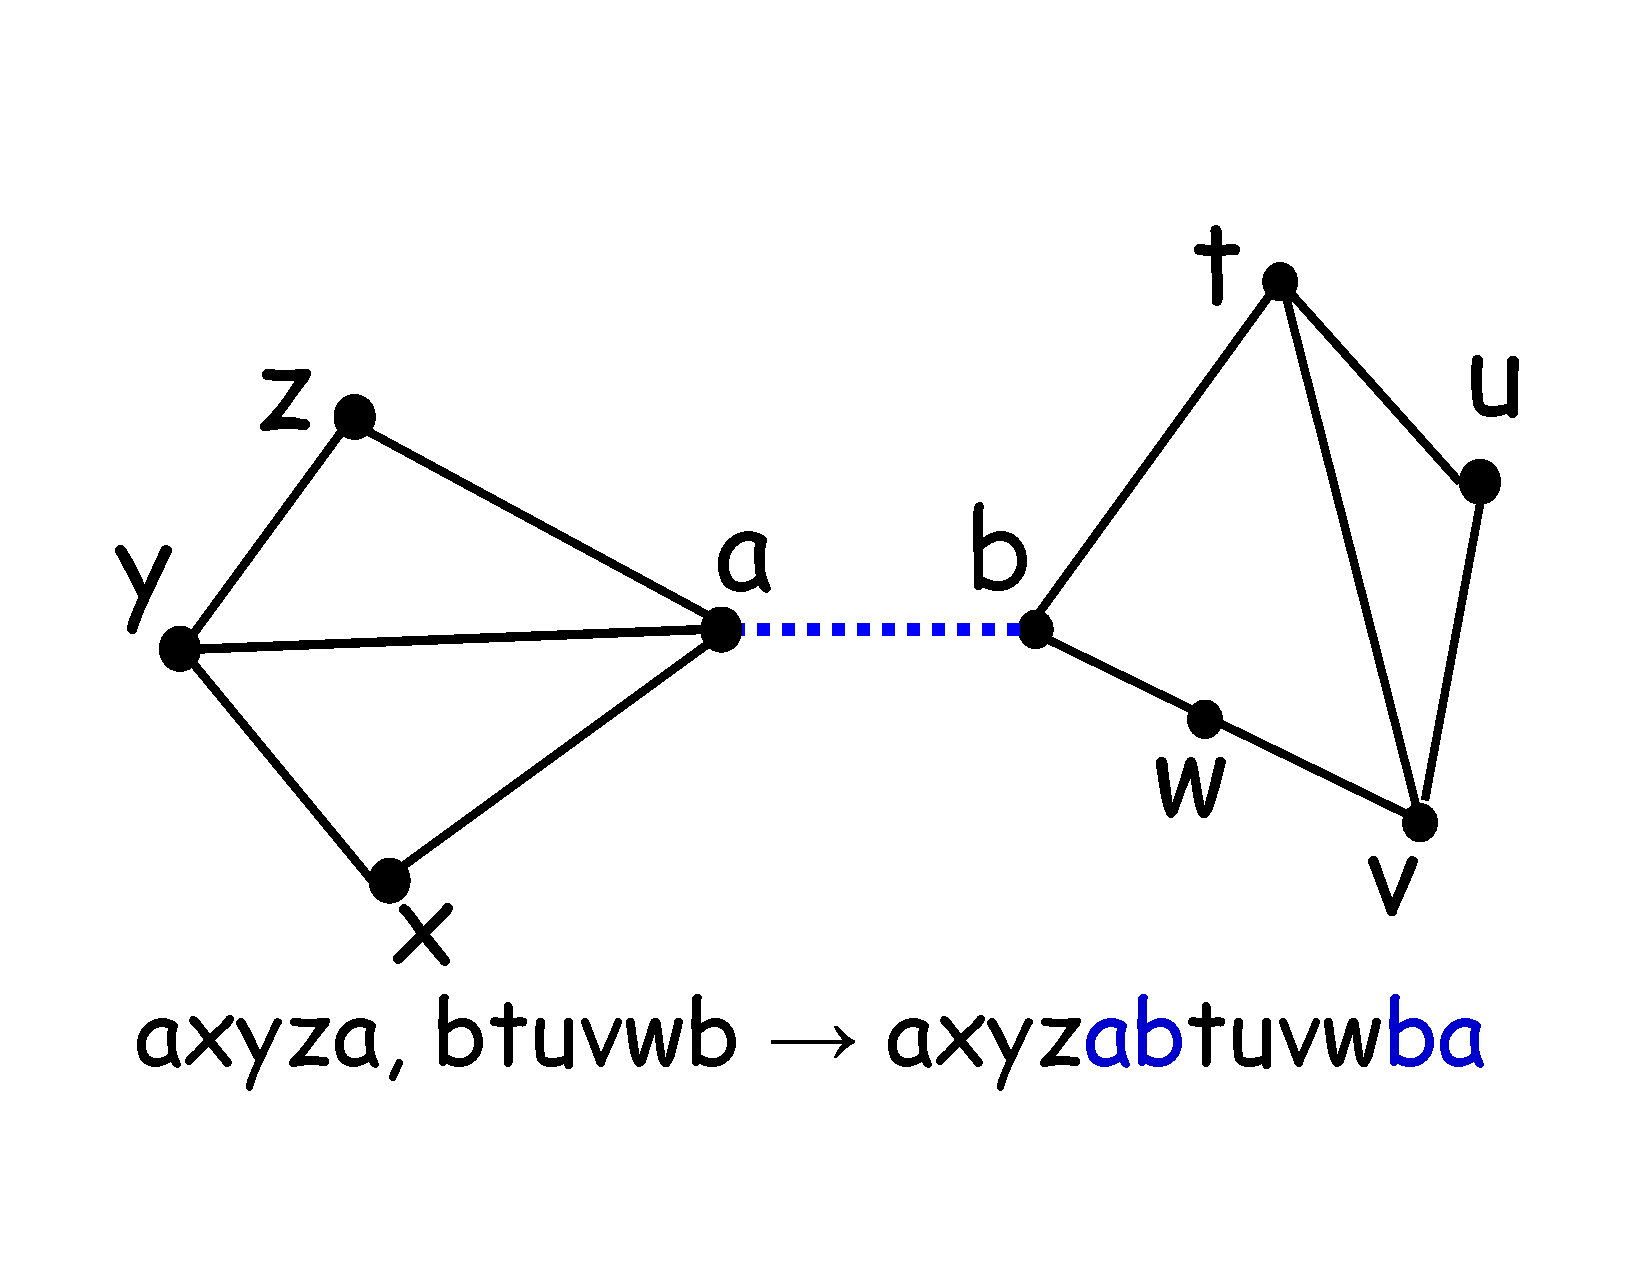
\includegraphics[height=3in]{figures/add-bridge}
\caption{The Add Bridge Case.}
\label{fig:add-bridge}
\end{figure}

\end{itemize}

An arbitrary graph is \term{planar} iff each of its connected components
has a planar embedding.

\end{definition}

\section{What \idx{outer face}?}
Notice that the definition of planar embedding does not distinguish an
``outer'' face.  There really isn't any need to distinguish one.

In fact, a planar embedding could be drawn with any given face on the
outside.  An intuitive explanation of this is to think of drawing the
embedding on a \emph{sphere} instead of the plane.  Then any face can be
made the outside face by ``puncturing'' that face of the sphere,
stretching the puncture hole to a circle around the rest of the faces,
and flattening the circular drawing onto the plane.

So pictures that show different ``outside'' boundaries may actually be
illustrations of the same planar embedding.

This is what justifies the ``add bridge'' case in a planar embedding:
whatever face is chosen in the embeddings of each of the disjoint planar
graphs, we can draw a bridge between them without needing to cross any
other edges in the drawing, because we can assume the bridge connects
two ``outer'' faces.

\section{Euler's Formula}

The value of the recursive definition is that it provides a powerful
technique for proving properties of planar graphs, namely, structural
induction.

One of the most basic properties of a connected planar graph is that its
number of vertices and edges determines the number of faces in every
possible planar embedding:

\begin{theorem}[\idx{Euler's Formula}]
If a connected graph has a planar embedding, then
%
\[
v - e + f = 2
\]
%
where $v$ is the number of vertices, $e$ is the number of edges, and
$f$ is the number of faces.
\end{theorem}

For example, in Figure~\ref{fig:continuous-faces}, $\card{V} = 4$,
$\card{E} = 6$, and $f = 4$.  Sure enough, $4 - 6 + 4 = 2$, as Euler's
Formula claims.

\begin{proof}
The proof is by structural induction on the definition of planar
embeddings.  Let $P(\embed{E})$ be the proposition that $v - e + f = 2$ for an
embedding, $\embed{E}$.

\textbf{Base case:} ($\embed{E}$ is the one vertex planar embedding).
By definition, $v=1$, $e=0$, and $f=1$, so $P(\embed{E})$ indeed holds.

\textbf{Constructor case:} (split a face) Suppose $G$ is a connected graph
with a planar embedding, and suppose $a$ and $b$ are distinct, nonadjacent
vertices of $G$ that appear on some discrete face,
$\gamma= a \dots b \cdots a$, of the planar embedding.

Then the graph obtained by adding the edge $\edge{a}{b}$ to the edges of
$G$ has a planar embedding with one more face and one more edge than $G$.
So the quantity $v-e+f$ will remain the same for both graphs, and since by
structural induction this quantity is 2 for $G$'s embedding, it's also 2
for the embedding of $G$ with the added edge.  So $P$ holds for the
constructed embedding.

\textbf{Constructor case:} (add bridge) Suppose $G$ and $H$ are connected
graphs with planar embeddings and disjoint sets of vertices.  Then
connecting these two graphs with a bridge merges the two bridged faces
into a single face, and leaves all other faces unchanged.  So the bridge
operation yields a planar embedding of a connected graph with $v_G +v_H$
vertices, $e_G + e_H +1$ edges, and $f_G + f_H - 1$ faces.  But
\begin{align*}
\lefteqn{(v_G +v_H) - (e_G + e_H +1) + (f_G + f_H - 1)}\\
   & = (v_G  - e_G + f_G) + (v_H  - e_H  + f_H) -2\\
   & = (2)+(2)-2 & \text{(by structural induction hypothesis)}\\
   & = 2.
\end{align*}
So $v-e+f$ remains equal to 2 for the constructed embedding.  That is, $P$
also holds in this case.

This completes the proof of the constructor cases, and the theorem follows
by structural induction.
\end{proof}

\iffalse
\mfigure{!}{1in}{figures/planar-assumptions.pdf}
\fi

\section{Number of Edges versus Vertices}

Like Euler's formula, the following lemmas follow by structural induction
directly from the definition of planar embedding.

\begin{lemma}\label{2e}
In a planar embedding of a connected graph, each edge is traversed once by
each of two different faces, or is traversed exactly twice by one face.
\end{lemma}

\begin{lemma}\label{3f}
  In a planar embedding of a connected graph with at least three vertices,
  each face is of length at least three.
\end{lemma}

\begin{corollary}\label{e3v}
Suppose a connected planar graph has $v \geq 3$ vertices and $e$ edges.
Then
\[
e \leq 3v-6.
\]
\end{corollary}

\begin{proof}
By definition, a connected graph is planar iff it has a planar embedding.
So suppose a connected graph with $v$ vertices and $e$ edges has a planar
embedding with $f$ faces.  By Lemma~\ref{2e}, every edge is traversed
exactly twice by the face boundaries.  So the sum of the lengths of the
face boundaries is exactly $2e$.  Also by Lemma~\ref{3f}, when $v \geq 3$,
each face boundary is of length at least three, so this sum is at least
$3f$.  This implies that
\begin{equation}\label{e3f}
3f \leq 2e.
\end{equation}
But $f = e-v+2$ by Euler's formula, and substituting into~\eqref{e3f} gives
\begin{align*}
3(e-v+2) & \leq 2e\\
e-3v + 6  & \leq 0\\
e & \leq 3v - 6
\end{align*}
\end{proof}

Corollary~\ref{e3v} lets us prove that the quadapi can't all shake hands
without crossing.  Representing quadapi by vertices and the necessary
handshakes by edges, we get the complete graph, \idx{$K_5$}.  Shaking
hands without crossing amounts to showing that $K_5$ is planar.  But $K_5$
is connected, has 5 vertices and 10 edges, and $10 > 3 \cdot 5-6$.  This
violates the condition of Corollary~\ref{e3v} required for $K_5$ to be
planar, which proves

\begin{lemma}\label{k5not}
$K_5$ is not planar.
\end{lemma}

Another consequence is
\begin{lemma}\label{d5}
Every planar graph has a vertex of degree at most five.
\end{lemma}

\begin{proof}
  If every vertex had degree at least 6, then the sum of the vertex
  degrees is at least $6v$, but since the sum equals $2e$, we have $e \geq
  3v$ contradicting the fact that $e \leq 3v-6 < 3v$ by
  Corollary~\ref{e3v}.
\end{proof}

\section{Planar Subgraphs}

If you draw a graph in the plane by repeatedly adding edges that don't
cross, you clearly could add the edges in any other order and still wind
up with the same drawing.  This is so basic that we might presume that our
recursively defined planar embeddings have this property.  But that
wouldn't be fair: we really need to prove it.  After all, the recursive
definition of planar embedding was pretty technical ---maybe we got it a
little bit wrong, with the result that our embeddings don't have this basic
draw-in-any-order property.

Now any ordering of edges can be obtained just by repeatedly switching the
order of successive edges, and if you think about the recursive definition
of embedding for a minute, you should realize that you can switch
\emph{any} pair of successive edges if you can just switch the last two.
So it all comes down to the following lemma.

\hyperdef{switch}{edges}{\begin{lemma}}\label{switch-edges} Suppose that,
  starting from some embeddings of planar graphs with disjoint sets of
  vertices, it is possible by two successive applications of constructor
  operations to add edges $e$ and then $f$ to obtain a planar embedding,
  $\embed{F}$.  Then starting from the same embeddings, it is also
  possible to obtain $\embed{F}$ by adding $f$ and then $e$ with two
  successive applications of constructor operations.
\end{lemma}

We'll leave the proof of Lemma~\ref{switch-edges} to
Problem~\ref{PS_planar_graph_construction_order}.

\begin{corollary}\label{permute-edges} Suppose that, starting from some
  embeddings of planar graphs with disjoint sets of vertices, it is
  possible to add a sequence of edges $e_0,e_1,\dots,e_n$ by successive
  applications of constructor operations to obtain a planar embedding,
  $\embed{F}$.  Then starting from the same embeddings, it is also
  possible to obtain $\embed{F}$ by applications of constructor operations
  that successively add any permutation\footnote{If $\pi:\set{0,1,\dots,n} \to
    \set{0,1,\dots,n}$ is a bijection, then the sequence
    $e_{\pi(0)},e_{\pi(1)},\dots,e_{\pi(n)}$ is called a \term{permutation} of
    the sequence $e_0,e_1,\dots,e_n$.} of the edges $e_0,e_1,\dots,e_n$.
\end{corollary}

\begin{corollary}\label{delete-edge}
Deleting an edge from a planar graph leaves a planar graph.

\begin{proof}
  By Corollary~\ref{permute-edges}, we may assume the deleted edge was the
  last one added in constructing an embedding of the graph.  So the
  embedding to which this last edge was added must be an embedding of the
  graph without that edge.
\end{proof}

\end{corollary}

Since we can delete a vertex by deleting all its incident edges,
Corollary~\ref{delete-edge} immediately implies

\begin{corollary}\label{delete-vertex}
Deleting a vertex from a planar graph, along with all its incident
edges of course, leaves another planar graph.
\end{corollary}

A \term{subgraph} of a graph, $G$, is any graph whose set of vertices is a
subset of the vertices of $G$ and whose set of edges is a subset of the
set of edges of $G$.  So we can summarize Corollaries~\ref{delete-edge}
and~\ref{delete-vertex} and their consequences in a Theorem.

\begin{theorem}\label{planar-subgraph}
  Any \index{planar subgraph}subgraph of a planar graph is planar.
\end{theorem}

\section{Planar \idx{5-Colorability}}

We need to know one more property of planar graphs in order to prove that
planar graphs are 5-colorable.

\begin{lemma}\label{mergelem}
Merging two adjacent vertices of a planar graph leaves another planar graph.
\end{lemma}

Here merging two adjacent vertices, $n_1$ and $n_2$ of a graph means
deleting the two vertices and then replacing them by a new ``merged''
vertex, $m$, adjacent to all the vertices that were adjacent to either of
$n_1$ or $n_2$, as illustrated in Figure~\ref{fig:merged}.

\begin{figure}%[h]
\centering 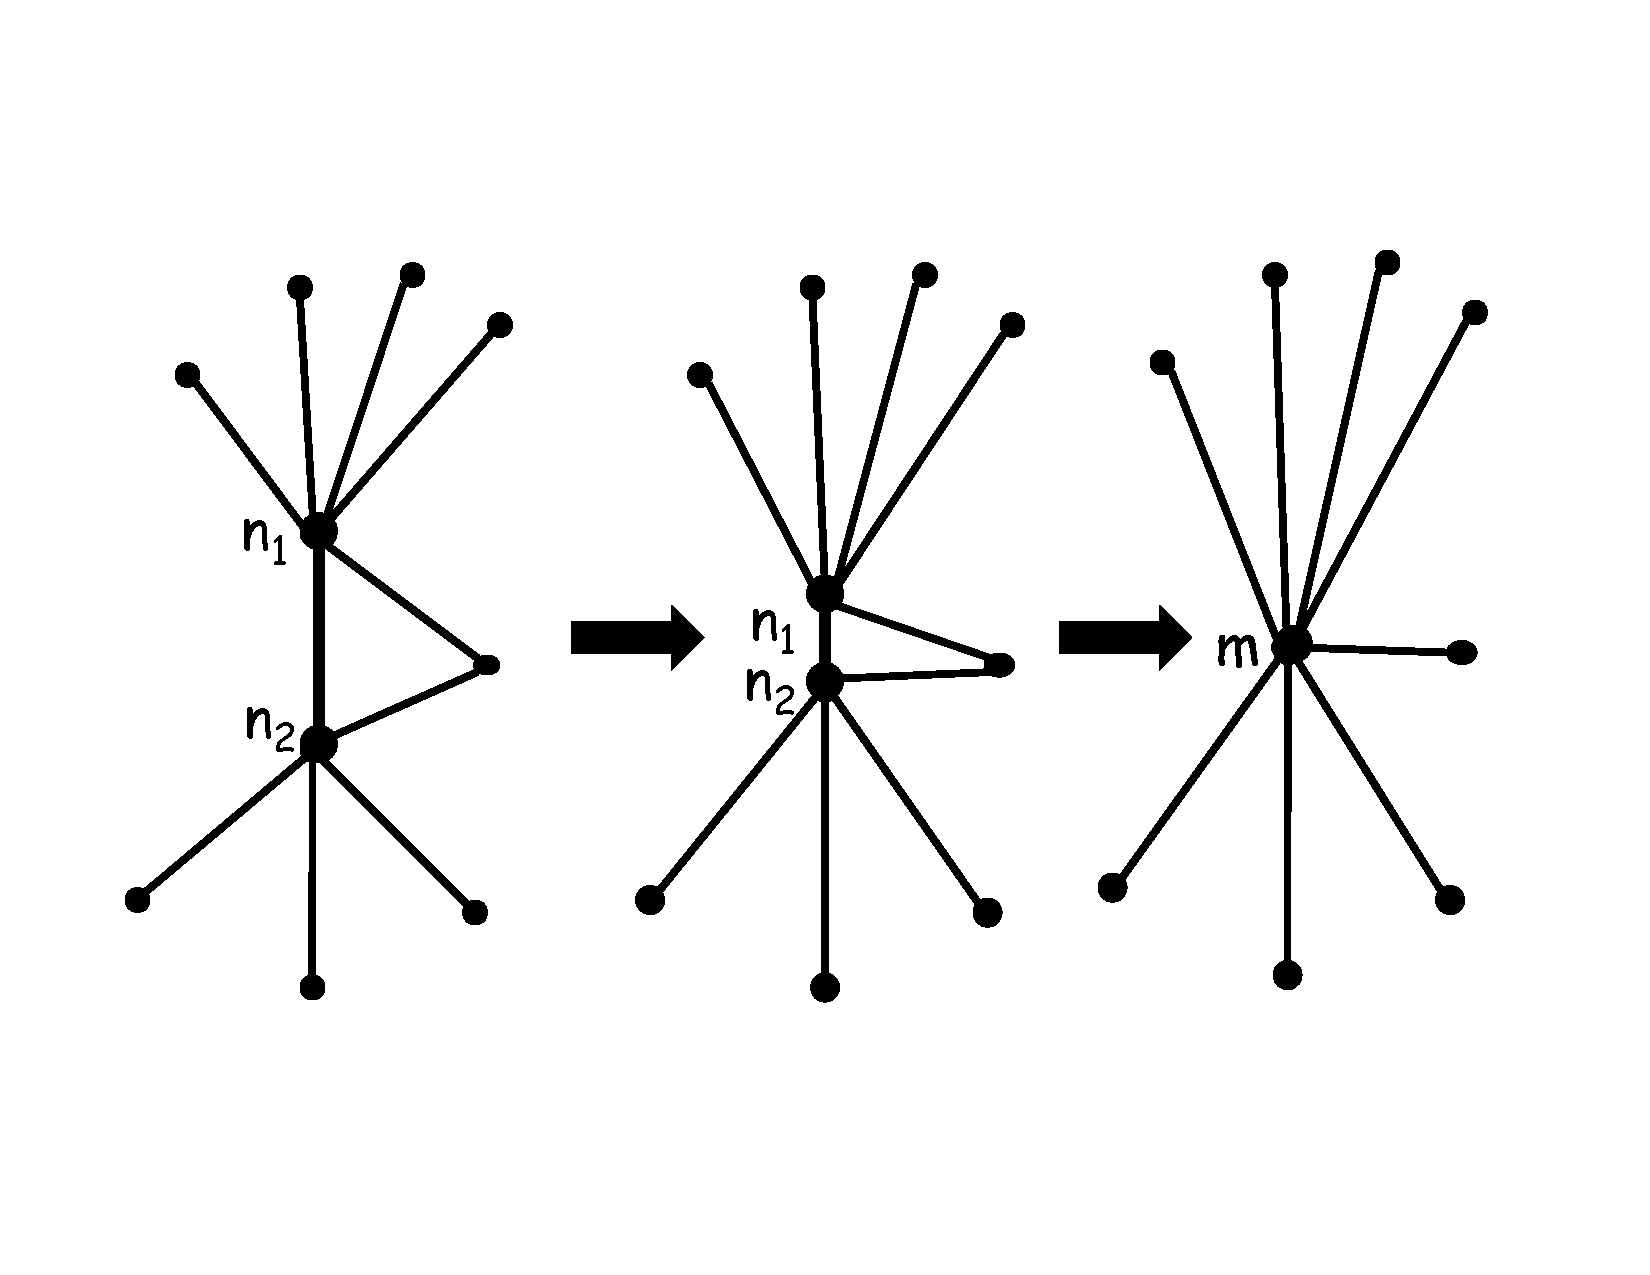
\includegraphics[height=4in]{figures/vertex-merge-arrows.pdf}
\caption{Merging adjacent vertices $n_1$ and $n_2$ into new vertex, $m$.}
\label{fig:merged}
\end{figure}

Lemma~\ref{mergelem} can be proved by structural induction, but the proof
is kind of boring, and we hope you'll be relieved that we're going to omit
it.  (If you insist, we can add it to the next problem set.)

Now we've got all the simple facts we need to prove 5-colorability.
\begin{theorem}
Every planar graph is five-colorable.
\end{theorem}

\begin{proof}
The proof will be by strong induction on the number, $v$, of vertices, with
induction hypothesis:
\begin{quote}
Every planar graph with $v$ vertices is five-colorable.
\end{quote}

\textbf{Base cases} ($v \leq 5$): immediate.

\textbf{Inductive case}: Suppose $G$ is a planar graph with $v+1$
vertices.  We will describe a five-coloring of $G$.

First, choose a vertex, $g$, of $G$ with degree at most 5; Lemma~\ref{d5}
guarantees there will be such a vertex.

\textbf{Case 1} ($\degr{g}<5$): Deleting $g$ from $G$ leaves a graph, $H$,
that is planar by Lemma~\ref{delete-vertex}, and, since $H$ has $v$ vertices,
it is five-colorable by induction hypothesis.  Now define a five coloring
of $G$ as follows: use the five-coloring of $H$ for all the vertices besides
$g$, and assign one of the five colors to $g$ that is not the same as the
color assigned to any of its neighbors.  Since there are fewer than 5
neighbors, there will always be such a color available for $g$.

\textbf{Case 2} ($\degr{g}=5$): If the five neighbors of $g$ in $G$ were
all adjacent to each other, then these five vertices would form a
nonplanar subgraph isomorphic to $K_5$, contradicting
Theorem~\ref{planar-subgraph}.  So there must be two neighbors, $n_1$ and
$n_2$, of $g$ that are not adjacent.  Now merge $n_1$ and $g$ into a new
vertex, $m$, as in Figure~\ref{fig:merged}.  In this new graph, $n_2$ is
adjacent to $m$, and the graph is planar by Lemma~\ref{mergelem}.  So we
can then merge $m$ and $n_2$ into a another new vertex, $m'$, resulting in
a new graph, $G'$, which by Lemma~\ref{mergelem} is also planar.  Now $G'$
has $v-1$ vertices and so is five-colorable by the induction hypothesis.

Now define a five coloring of $G$ as follows: use the five-coloring of $G'$
for all the vertices besides $g$, $n_1$ and $n_2$.  Next assign the color
of $m'$ in $G'$ to be the color of the neighbors $n_1$ and $n_2$.  Since
$n_1$ and $n_2$ are not adjacent in $G$, this defines a proper
five-coloring of $G$ except for vertex $g$.  But since these two neighbors
of $g$ have the same color, the neighbors of $g$ have been colored using
fewer than five colors altogether.  So complete the five-coloring of $G$ by
assigning one of the five colors to $g$ that is not the same as any of the
colors assigned to its neighbors.

\end{proof}

A graph obtained from a graph, $G$, be repeatedly deleting vertices,
deleting edges, and merging adjacent vertices is called a \term{minor} of
$G$.  Since \idx{$K_5$} and \idx{$K_{3,3}$} are not planar,
Lemmas~\ref{delete-edge},~\ref{delete-vertex}, and~\ref{mergelem}
immediately imply:

\begin{corollary}\label{forbiddenK}
  A graph which has $K_5$ or $K_{3,3}$ as a minor is not planar.
\end{corollary}

We don't have time to prove it, but the converse of
Corollary~\ref{forbiddenK} is also true.  This gives the following famous,
very elegant, and purely discrete characterization of planar graphs:

\begin{theorem}[\idx{Kuratowksi}]
  A graph is not planar iff it has $K_5$ or $K_{3,3}$ as a minor.
\end{theorem}

\section{Classifying \idx{Polyhedra}}

The \idx{Pythagoreans} had two great mathematical secrets, the
irrationality of $\sqrt{2}$ and a geometric construct that we're about to
rediscover!

A \term{polyhedron} is a convex, three-dimensional region bounded by a
finite number of polygonal faces.  If the faces are identical regular
polygons and an equal number of polygons meet at each corner, then the
polyhedron is \index{regular polyhedron}\term*{regular}.  Three examples
of regular polyhedra are shown below: the tetrahedron, the cube, and the
octahedron.

\mfigure{!}{1.25in}{figures/polyhedra.pdf}

We can determine how many more regular polyhedra there are by thinking
about planarity.  Suppose we took \emph{any} polyhedron and placed a
sphere inside it.  Then we could project the polyhedron face boundaries
onto the sphere, which would give an image that was a planar graph
embedded on the sphere, with the images of the corners of the polyhedron
corresponding to vertices of the graph.  But we've already observed that
embeddings on a sphere are the same as embeddings on the plane, so Euler's
formula for planar graphs can help guide our search for regular polyhedra.

For example, planar embeddings of the three polyhedra above look like
this:

%\mfigure{!}{1.25in}{figures/polyhedra-blowup.pdf}
\begin{center}
\setlength{\unitlength}{2000sp}%{3947sp}%
%
\begingroup\makeatletter\ifx\SetFigFont\undefined%
\gdef\SetFigFont#1#2#3#4#5{%
  \reset@font\fontsize{#1}{#2pt}%
  \fontfamily{#3}\fontseries{#4}\fontshape{#5}%
  \selectfont}%
\fi\endgroup%
\begin{picture}(9999,2124)(1489,-3073)
%\thinlines
{\color[rgb]{0,0,0}\put(8476,-3061){\line( 3, 4){1548}}
\put(9976,-961){\line( 3,-4){1548}}
\put(11476,-3061){\line(-1, 0){3000}}
}%
{\color[rgb]{0,0,0}\put(9526,-2011){\line( 1, 0){900}}
\put(10426,-2011){\line(-3,-5){450}}
\put(9976,-2761){\line(-3, 5){450}}
}%
{\color[rgb]{0,0,0}\put(8476,-3061){\line( 1, 1){1050}}
\put(9526,-2011){\line( 2, 5){424.138}}
}%
{\color[rgb]{0,0,0}\put(9976,-961){\line( 2,-5){424.138}}
\put(10426,-2011){\line( 1,-1){1050}}
}%
{\color[rgb]{0,0,0}\put(11476,-3061){\line(-5, 1){1500}}
\put(9976,-2761){\line(-5,-1){1500}}
}%
{\color[rgb]{0,0,0}\put(3001,-1261){\line(-5,-6){1500}}
\put(1501,-3061){\line( 1, 0){3000}}
\put(4501,-3061){\line(-5, 6){1500}}
\put(3001,-1261){\line( 0,-1){1200}}
\put(3001,-2461){\line(-5,-2){1500}}
}%
{\color[rgb]{0,0,0}\put(3001,-2461){\line( 5,-2){1500}}
}%
{\color[rgb]{0,0,0}\put(5401,-3061){\framebox(2100,2100){}}
}%
{\color[rgb]{0,0,0}\put(6001,-2461){\framebox(900,900){}}
}%
{\color[rgb]{0,0,0}\put(5401,-961){\line( 1,-1){600}}
}%
{\color[rgb]{0,0,0}\put(5401,-3061){\line( 1, 1){600}}
}%
{\color[rgb]{0,0,0}\put(7501,-3061){\line(-1, 1){600}}
}%
{\color[rgb]{0,0,0}\put(7501,-961){\line(-1,-1){600}}
}%
\end{picture}%

\end{center}

Let $m$ be the number of faces that meet at each corner of a
polyhedron, and let $n$ be the number of sides on each face.  In the
corresponding planar graph, there are $m$ edges incident to each of
the $v$ vertices.  Since each edge is incident to two vertices, we
know:
%
\[
m v = 2 e
\]
%
Also, each face is bounded by $n$ edges.  Since each edge is on the
boundary of two faces, we have:
%
\[
n f = 2 e
\]
%
Solving for $v$ and $f$ in these equations and then substituting into
\idx{Euler's formula} gives:
\[
\frac{2e}{m} - e + \frac{2e}{n} = 2
\]
which simplifies to
\begin{equation}\label{1m1n}
\frac{1}{m} + \frac{1}{n} = \frac{1}{e} + \frac{1}{2}
\end{equation}
%
This last equation~\eqref{1m1n} places strong restrictions on the
structure of a polyhedron.  Every nondegenerate polygon has at least 3
sides, so $n \geq 3$.  And at least 3 polygons must meet to form a corner,
so $m \geq 3$.  On the other hand, if either $n$ or $m$ were 6 or more,
then the left side of the equation could be at most $1/3 + 1/6 = 1/2$,
which is less than the right side.  Checking the finitely-many cases that
remain turns up only five solutions.  For each valid combination of $n$
and $m$, we can compute the associated number of vertices $v$, edges $e$,
and faces $f$.  And polyhedra with these properties do actually exist:
%
\[
\begin{array}{cc|ccc|l}
n & m & v  & e  &  f & \text{polyhedron} \\ \hline
3 & 3 & 4  & 6  &  4 & \text{tetrahedron} \\
4 & 3 & 8  & 12 &  6 & \text{cube} \\
3 & 4 & 6  & 12 &  8 & \text{octahedron} \\
3 & 5 & 12 & 30 & 20 & \text{icosahedron} \\
5 & 3 & 20 & 30 & 12 & \text{dodecahedron}
\end{array}
\]
%
The last polyhedron in this list, the dodecahedron, was the other great
mathematical secret of the Pythagorean sect.  These five, then, are the
only possible regular polyhedra.

So if you want to put more than 20 geocentric satellites in orbit so that
they \emph{uniformly} blanket the globe ---tough luck!

%% Planar Graphs Problems %%%%%%%%%%%%%%%%%%%%%%%%%%%%%%%%%%%%%%%%%%%%%%%%%%%%%
\begin{problems}

\examproblems
\pinput{MQ_planar_isomorphism}

\classproblems
\pinput{CP_planar_embedding_isomorphism}
\pinput{CP_K33_not_planar}
\pinput{CP_planar_structural_induction}

\homeworkproblems  
\pinput{PS_triangle_free_planar_graphs}
\pinput{PS_planar_graph_construction_order}

%\pinput{CP0506_}
\end{problems}

%% Conclusion %%%%%%%%%%%%%%%%%%%%%%%%%%%%%%%%%%%%%%%%%%%%%%%%%%%%%%%%%%%%%%%%%
%\TBA{Add conclusion here...}

\endinput
